\chapter{Planen}\label{ch:planen}
In diesem Abschnitt, wird die Planung beschrieben. In dieser Phase werden basierend auf den Anforderungen Arbeitspakete erstellt, und in einem GANT-Diagramm auf die 10 Tage eingeteilt.

\section{Arbeitspakete}

Um den ganzen Auftrag in kleine übersichtliche Teile aufzuteilen, wird er in verschiedene kleine Arbeitspakete unterteilt. Die Arbeitspakete sind jeweils nummeriert, haben einen Namen, einen geschätzten Aufwand in Stunden und eine \flqq Definition of Done\frqq{}/ ein erwartetes Ergebnis. Die Aufwände sind oft mit einem gewissen Puffer geschätzt.\\
Die Pakete  sind nach den 6 Phasen der IPERKA Methode aufgelistet. Arbeiten welche IPA-spezifisch sind, werden unter Rahmenaufgaben aufgeführt.

\subsection{Informieren}
Hier, sind die Arbeitspakete, welche während der IPERKA-Phase \flqq Informieren\frqq{}\space bearbeitet wurden, aufgelistet.

\begin{longtable}{p{.22\textwidth}|p{.78\textwidth}}
	\hline
	\textbf{Nummer}    				& 1.1 \\
	\hline
	\textbf{Name}   				& Projektumfeld analysieren und beschreiben \\
	\hline
	\textbf{Geschätzter Aufwand}	& 2h \\
	\hline
	\textbf{Erwartetes Ergebnis}	& Das Ziel der Arbeit ist klar und ein grober Überblick besteht. \\
	\hline
\end{longtable}

\begin{longtable}{p{.22\textwidth}|p{.78\textwidth}}
	\hline
	\textbf{Nummer}    				& 1.2 \\
	\hline
	\textbf{Name}   				& Anforderungen definieren \\
	\hline
	\textbf{Geschätzter Aufwand}	& 2h \\
	\hline
	\textbf{Erwartetes Ergebnis}	& Die funktionalen und nicht-funktionalen Anforderungen sind definiert und beschrieben.\\
	\hline
\end{longtable}\pagebreak

\subsection{Planen}
Hier, sind die Arbeitspakete, welche während der IPERKA-Phase \flqq Planen\frqq{}\space bearbeitet werden, aufgelistet.

\begin{longtable}{p{.22\textwidth}|p{.78\textwidth}}
	\hline
	\textbf{Nummer}    				& 2.1 \\
	\hline
	\textbf{Name}   				& Arbeitspakete definieren \\
	\hline
	\textbf{Geschätzter Aufwand}	& 3h \\
	\hline
	\textbf{Erwartetes Ergebnis}	& Die ganze Arbeit ist in kleine logische Arbeitspakete unterteilt. Alle Arbeitspakete sind klar definiert.\\
	\hline
\end{longtable}

\begin{longtable}{p{.22\textwidth}|p{.78\textwidth}}
	\hline
	\textbf{Nummer}    				& 2.2 \\
	\hline
	\textbf{Name}   				& Zeitplan erstellen \\
	\hline
	\textbf{Geschätzter Aufwand}	& 1h \\
	\hline
	\textbf{Erwartetes Ergebnis}	& Der GANT-Zeitplan ist anhand der Arbeitspakete erstellt. Es sind alle Arbeitspakete auf dem Zeitplan vorhanden.\\
	\hline
\end{longtable}

\begin{longtable}{p{.22\textwidth}|p{.78\textwidth}}
	\hline
	\textbf{Nummer}    				& 2.3 \\
	\hline
	\textbf{Name}   				& Lösungskonzept für das Backend erarbeiten\\
	\hline
	\textbf{Geschätzter Aufwand}	& 4h \\
	\hline
	\textbf{Erwartetes Ergebnis}	& Es ist mindestens ein Lösungsvorschlag definiert und so weit wie Sinnvoll beschrieben und durchgedacht. Der relevante Backendcode ist verstanden.\\
	\hline
\end{longtable}\pagebreak

\begin{longtable}{p{.22\textwidth}|p{.78\textwidth}}
	\hline
	\textbf{Nummer}    				& 2.4 \\
	\hline
	\textbf{Name}   				& Lösungskonzept für die SPA erarbeiten\\
	\hline
	\textbf{Geschätzter Aufwand}	& 4h \\
	\hline
	\textbf{Erwartetes Ergebnis}	& Es ist mindestens ein Lösungsvorschlag definiert und so weit wie Sinnvoll beschrieben und durchgedacht. Es sind verschiedene Mockups vorhanden, und der relevante SPA Code ist verstanden.\\
	\hline
\end{longtable}

\begin{longtable}{p{.22\textwidth}|p{.78\textwidth}}
	\hline
	\textbf{Nummer}    				& 2.5 \\
	\hline
	\textbf{Name}   				& Test- und Qualitätssicherungskonzept erstellen\\
	\hline
	\textbf{Geschätzter Aufwand}	& 4h \\
	\hline
	\textbf{Erwartetes Ergebnis}	& Das Testkonzept ist erstellt und dokumentiert. Das Qualitätssicherungskonzept ist erstellt und dokumentiert.\\
	\hline
\end{longtable}

\subsection{Entscheiden}
Hier, sind die Arbeitspakete, welche während der IPERKA-Phase \flqq Entscheiden\frqq{}\space bearbeitet werden, aufgelistet.

\begin{longtable}{p{.22\textwidth}|p{.78\textwidth}}
	\hline
	\textbf{Nummer}    				& 3.1 \\
	\hline
	\textbf{Name}   				& Lösungsvarianten evaluieren \\
	\hline
	\textbf{Geschätzter Aufwand}	& 2h \\
	\hline
	\textbf{Erwartetes Ergebnis}	& Aus den verschiedenen Lösungsvarianten der SPA und des Backends wurde sich für eine entschieden. Die Entscheidung ist begründet dokumentiert.\\
	\hline
\end{longtable}\pagebreak

\subsection{Realisieren}
Hier, sind die Arbeitspakete, welche während der IPERKA-Phase \flqq Realisieren\frqq{}\space bearbeitet werden, aufgelistet.

\begin{longtable}{p{.22\textwidth}|p{.78\textwidth}}
	\hline
	\textbf{Nummer}    				& 4.1 \\
	\hline
	\textbf{Name}   				& Das Backend erweitern  \\
	\hline
	\textbf{Geschätzter Aufwand}	& 14h \\
	\hline
	\textbf{Erwartetes Ergebnis}	& Alle Anforderungen für das Backend sind nach dem definierten Lösungsansatz umgesetzt. Die Lösung ist vollständig dokumentiert. \\
	\hline
\end{longtable}

\begin{longtable}{p{.22\textwidth}|p{.78\textwidth}}
	\hline
	\textbf{Nummer}    				& 4.2 \\
	\hline
	\textbf{Name}   				& Unit- und Integration-Tests schreiben  \\
	\hline
	\textbf{Geschätzter Aufwand}	& 6h \\
	\hline
	\textbf{Erwartetes Ergebnis}	& Alle neuen Funktionalitäten sind mit Unit- und/oder Integration-Tests getestet.\\
	\hline
\end{longtable}


\begin{longtable}{p{.22\textwidth}|p{.78\textwidth}}
	\hline
	\textbf{Nummer}    				& 4.3 \\
	\hline
	\textbf{Name}   				& Die SPA erweitern  \\
	\hline
	\textbf{Geschätzter Aufwand}	& 6h \\
	\hline
	\textbf{Erwartetes Ergebnis}	& Alle Anforderungen für die SPA sind nach dem definierten Lösungsansatz umgesetzt. Die Lösung ist vollständig dokumentiert.\\
	\hline
\end{longtable}

\begin{longtable}{p{.22\textwidth}|p{.78\textwidth}}
	\hline
	\textbf{Nummer}    				& 4.4 \\
	\hline
	\textbf{Name}   				& Selenium Integration-Tests implementieren  \\
	\hline
	\textbf{Geschätzter Aufwand}	& 5h \\
	\hline
	\textbf{Erwartetes Ergebnis}	& Alle neuen Funktionalitäten sind mit Selenium Integration-Tests getestet.\\
	\hline
\end{longtable}\pagebreak

\begin{longtable}{p{.22\textwidth}|p{.78\textwidth}}
	\hline
	\textbf{Nummer}    				& 4.5 \\
	\hline
	\textbf{Name}   				& Kundendokumentation schreiben  \\
	\hline
	\textbf{Geschätzter Aufwand}	& 2h \\
	\hline
	\textbf{Erwartetes Ergebnis}	& Die neue Funktionalität ist in der Kundendokumentation dokumentiert, und alle Anforderungen sind erfüllt.\\
	\hline
\end{longtable}


\subsection{Kontrollieren}
Hier, sind die Arbeitspakete, welche während der IPERKA-Phase \flqq Kontrollieren\frqq{}\space bearbeitet werden, aufgelistet.

\begin{longtable}{p{.22\textwidth}|p{.78\textwidth}}
	\hline
	\textbf{Nummer}    				& 5.1 \\
	\hline
	\textbf{Name}   				& Tests durchführen, und Fehler beheben \\
	\hline
	\textbf{Geschätzter Aufwand}	& 4h \\
	\hline
	\textbf{Erwartetes Ergebnis}	& Tests sind gemäss Testkonzept durchgeführt, und mögliche Fehler sind behoben. \\
	\hline
\end{longtable}

\begin{longtable}{p{.22\textwidth}|p{.78\textwidth}}
	\hline
	\textbf{Nummer}    				& 5.2 \\
	\hline
	\textbf{Name}   				& Codequalität prüfen, und Refactorn \\
	\hline
	\textbf{Geschätzter Aufwand}	& 1h \\
	\hline
	\textbf{Erwartetes Ergebnis}	& Code ist nochmals durchgeschaut, und Unschönheiten sind bereinigt.\\
	\hline
\end{longtable}

\begin{longtable}{p{.22\textwidth}|p{.78\textwidth}}
	\hline
	\textbf{Nummer}    				& 5.3 \\
	\hline
	\textbf{Name}   				& Dokumentation finalisieren \\
	\hline
	\textbf{Geschätzter Aufwand}	& 8h \\
	\hline
	\textbf{Erwartetes Ergebnis}	& Die Dokumentation ist soweit wie möglich finalisiert und entspricht den Vorgaben.\\
	\hline
\end{longtable}

\subsection{Auswerten}
Hier, sind die Arbeitspakete, welche während der letzten IPERKA-Phase \flqq Auswerten\frqq{}\space bearbeitet werden, aufgelistet.

\begin{longtable}{p{.22\textwidth}|p{.78\textwidth}}
	\hline
	\textbf{Nummer}    				& 6.2 \\
	\hline
	\textbf{Name}   				& Reflexion schreiben \\
	\hline
	\textbf{Geschätzter Aufwand}	& 2h \\
	\hline
	\textbf{Erwartetes Ergebnis}	& Reflexion zu der Arbeit ist geschrieben. \\
	\hline
\end{longtable}

\subsection{Rahmenaufgaben}
Hier, sind die Arbeitspakete, welche IPA-spezifische Arbeit erfordern, aufgelistet.

\begin{longtable}{p{.22\textwidth}|p{.78\textwidth}}
	\hline
	\textbf{Nummer}    				& 7.1 \\
	\hline
	\textbf{Name}   				& Projektstruktur aufsetzen\\
	\hline
	\textbf{Geschätzter Aufwand}	& 2h \\
	\hline
	\textbf{Erwartetes Ergebnis}	& Das Grundgerüst für den Bericht steht. Der Latex-Build ist lauffähig und generiert ein anschaubares PDF.\\
	\hline
\end{longtable}

\begin{longtable}{p{.22\textwidth}|p{.78\textwidth}}
	\hline
	\textbf{Nummer}    				& 7.2 \\
	\hline
	\textbf{Name}   				& Aufgabenstellung und Rahmenbedingungen beschreiben\\
	\hline
	\textbf{Geschätzter Aufwand}	& 1h \\
	\hline
	\textbf{Erwartetes Ergebnis}	& Die Aufgabenstellung ist in den Bericht übernommen. Benützte Firmenstandarts sowie die Projektaufbauorganisation sind defniert und beschrieben. \\
	\hline
\end{longtable}

\newpage

\begin{longtable}{p{.22\textwidth}|p{.78\textwidth}}
	\hline
	\textbf{Nummer}    				& 7.3 \\
	\hline
	\textbf{Name}   				& Projektmanagementmethode definieren\\
	\hline
	\textbf{Geschätzter Aufwand}	& 1h \\
	\hline
	\textbf{Erwartetes Ergebnis}	& Es steht fest mit welcher Projektmanagementmethode die Probe-IPA umgesetzt werden soll. Der Bericht wurde so gegliedert.\\
	\hline
\end{longtable}

\begin{longtable}{p{.22\textwidth}|p{.78\textwidth}}
	\hline
	\textbf{Nummer}    				& 7.4 \\
	\hline
	\textbf{Name}   				& Expertenbesuche\\
	\hline
	\textbf{Geschätzter Aufwand}	& 4h \\
	\hline
	\textbf{Erwartetes Ergebnis}	& Infos aus dem Gespräch sind am richtigen Ort festgehalten.\\
	\hline
\end{longtable}

\begin{longtable}{p{.22\textwidth}|p{.78\textwidth}}
	\hline
	\textbf{Nummer}    				& 7.5 \\
	\hline
	\textbf{Name}   				& Anhang erstellen\\
	\hline
	\textbf{Geschätzter Aufwand}	& 2h \\
	\hline
	\textbf{Erwartetes Ergebnis}	& Der Anhang ist erstellt und beinhaltet alle nötigen und verlangten Inhalte.\\
	\hline
\end{longtable} 
\newpage

\section{Lösungskonzept Backend}

In diesem Kapitel ist das Lösungskonzept für das Backend beschrieben. Das Konzept richtet sich nach den in Kapitel \ref{subsec:anforderungenBackend} definierten Anforderungen. Es wurden diverse TODO's im Code hinzugefügt, dies macht die Implementation danach etwas effizienter.

\subsection{REST}\label{subsec:rest}

Damit die SPA den 16-stelligen Aktivierungscode anzeigen kann, muss er mit Hilfe einer REST-Schnittstelle übermittelt werden. Dass er aber überhaupt von Futurae erstellt wird, muss er bei dem Enrollement, also dem Call der einen neuen Nutzer erstellt, explizit gefordert werden. 
Dies funktioniert in dem man den Requestparameter \flqq short\_code\frqq{} auf true setzt. Für die Übermittlung dieser Information an die SPA stehen 2 Optionen im Raum:

\begin{itemize}
	\item Option 1: Den Endpunkt, welcher alle Accountdaten von jedem Nutzer zurückgibt um den Activation Code erweitern. Dies hätte zur Folge das der Endpunkt um ein optionales Feld \flqq activation\_code\_short\frqq{}\space erweitert wird.
	\label{"itm:restOption1"}
	\item Option 2: Einen neuen Endpunkt erstellen, welcher den offenen Aktivierungscode zurück gibt. Dies wäre ein einfacher GET-Endpunkte, welcher, falls vorhanden den neusten, ausstehenden Aktivierungscode zurück gibt. Folgend eine kurze Spezifikation des Endpunktes:\\\\

	\textbf{Pfad:} /auth-admin/rest/users/{userId}/tokens/airlock-2fa/activation-code-short\\
	\textbf{HTTP-Methode:} GET\\
	\textbf{Pfadparameter:} userid\\
	\textbf{Response:} Optionaler Actiovation Code, kann leer sein \newline
	\textbf{Status Codes:}
	\begin{longtable}{p{.25\textwidth}|p{.55\textwidth}}
		\hline
		\textbf{200 Ok}    				& 16-stelliger Aktivierungscode oder eine leere Response \\
		\hline
		\textbf{401 Unauthorized}   				& Invalide oder fehlende Authentifizierung\\
		\hline
		\textbf{403 Forbidden}	& Der Zugriff ist verboten (z.B bei fehlender oder falscher Adminrolle) \\
		\hline
		\textbf{404 Not Found}	& Mögliche Error Codes:
		\begin{itemize}
			\item USER\_NOT\_FOUND 
			\item ACCOUNT\_NOT\_FOUND
		\end{itemize}\\
		\hline
	\end{longtable} 
	
	\label{"itm:restOption2"}	
\end{itemize}

In beiden Fällen müsste der Restflow so aussehen:
\begin{figure}[H]
	\begin{center}
		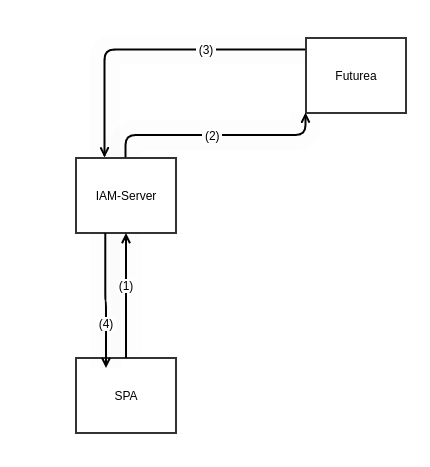
\includegraphics[width=0.8\textwidth]{ressourcen/restflow}
		\caption[Restflow]{Restflow um 16-stelligen Aktivierungscode zu bekommen}\label{fig:restflow}
	\end{center}
\end{figure}

\begin{itemize}
	\item[(1)] Die SPA macht als Reaktion auf einen Klick einen Request, ans IAM-Backend. Je nach Option, geht dieser an einen anderen Endpunkt. 
	\item[(2)] Das Backend macht folgenden Request an Futurae: \newline
	/srv/admin/v1/enrollments?status=pending
	\item[(3)] 	Da, bei dem Enrollment Request zu Futurae der 16-stellige Aktivierungscode explizit gefordert wurde, wird dieser Request, falls überhaupt ein austehendes Enrollment vorhanden ist, dieses auch zurück geben. Da mehrere offene Enrollments vorhanden sein können, muss immer das Neuste genommen werden. So ist immer klar um welchen 16-stelligen Aktivierungscode es sich handelt. Helpdesk oder Schalter Mitarbeiter können so die Aktivierung direkt mit dem Kunden durchspielen.
	\item[(4)] Das Backend gibt den Aktivierungscode an die SPA weiter. Je nach Option auch noch die anderen Accountdaten. Falls keiner vorhanden ist, wird das Feld in der Response einfach leer gelassen.
\end{itemize}


\subsection{Rollenlogik}
Es gibt bereits eine Regel, welche das Ansehen von Airlock 2FA Aktivierungsdaten einschränkt. Diese Regel kann wiederverwendet werden. Dazu gibt es einen \flqq Airlock2FAAccessController.java.\frqq{} Dieser kann beim erstellen der Response injected werden. Mit der Methode \flqq isAllowedToSeeActivationSecrets\frqq{} \space kann dann überprüft werden, ob der Adminnutzer diese Info überhaupt sehen darf. Am besten wird dieser Check noch vor dem Futurae Request ausgeführt, um einen unnötigen Rountrip zu vermeiden und es möglichst effizient zu halten. Falls die Option mit einem neuen Endpunkt gewählt wird, kann dieser separat geschützt werden, dann fällt die Logik mit dem \flqq Airlock2FAAccessController.java.\frqq{} weg.

\subsection{Wichtige Klassen und Interfaces}
\textbf{Option 1}
\begin{itemize}
	\item UserAirlock2FADeviceResource.java: In dieser Klasse befindet sich der GET-Endpunkt \flqq /auth-admin/rest/users/{userId}/tokens/airlock-2fa \frqq{}, welcher erweitert werden muss. 
	\item Airlock2FAUserAccount.java dies ist die Klasse welche die wichtigen Daten über den Acount beinhaltet. Diese Klasse muss um das Feld \flqq activationCodeShort\frqq{} erweitert werden.
	\item Airlock2FAAdminService.java: Dieser Service wird aus der Resource aufgerufen, um den Account von der Datenbank zu bekommen.
	\item Airlock2FAUserAccountRepository.java: Das Repository ist die Schnittstelle zwischen der Datenbank und dem Service. Die darin enthaltene \flqq findBy()\frqq{} Methode gibt schluss endlich den zusammengestellten \flqq Airlock2FAUserAccount.java\frqq{} zurück.
\end{itemize}
\textbf{Option 2}
\begin{itemize}
	\item UserAirlock2FADeviceResource.java: In dieser Klasse wird der oben definierte Endpunkt \flqq /auth-admin/rest/users/{userId}/tokens/airlock-2fa/activation-code-short \frqq{} erstellt.
	\item Airlock2FAAdminService.java: Dieser Service wird aus der Resource aufgerufen, hier muss eine neue Methode erstellt werden, welche den 16-stelligen Aktivierungscode, via dem <<FuturaeAdminApiEnrollmentServiceImpl.java>>, der Resource zur Verfügung stellt.
\end{itemize}
\textbf{Request zu Futurae}\newline
Der Request zu Futurae wird in beiden Optionen gleich aussehen. Lediglich der \flqq FuturaeAdminApiEnrollmentServiceImpl.java\frqq{} wird an verschiedenen Orten gebraucht.
\begin{itemize}
	\item FuturaeAdminApiEnrollmentServiceImpl.java: In diesem Serivce muss der\\ Airlock2FAAccessController injected werden. Zusätzlich wird es eine neue Methode geben müssen, welche zuerst mit Hilfe des Airlock2FAAccessController prüft, ob der Adminnutzer die richtige Rolle hat. Danach wird via die \flqq FuturaeAdminApiEnrollmentRequestFactory.java\frqq{} der Request zusammengestellt. Dieser Request wird dann via den RestClient ausgeführt. Die Response wird dann in ein neu erstelltes ...Response Objekt gespeichert und zurück gegeben. 
	\item FuturaeAdminApiEnrollmentRequestFactory.java: In dieser Klasse braucht es eine neue Methode welche einen Request zusammenstellt, der von Futurae die neueste offene Aktivierung anfragt.
	\item AdminEnrollmentRequest.java: Diese Klasse bildet den Admin-Request ab, welcher gesendet wird, um neue Geräte zu aktivieren. Er muss um das Feld \flqq short\_code\frqq{} erweitert werden. Dieses Feld muss anschliessend für jeden Enrolloment-Request auf true gestzt werden.
	\item FuturaeAuthApiEnrollmentRequestFactory.java: Es ist wichtig auch in dieser Klasse auf dem Enrollmentrequest \flqq short\_code\frqq{} auf true zu setzen, ansonsten wird der 16-stellige Aktivierungscode nicht erzwungen, wenn das Enrollment von einem Endnutzer aus dem Self-Service gestartet wrid. Denn dann verläuft es über die Auth API. 
\end{itemize}



\section{Lösungskonzept SPA}\label{sec:lk-spa}
In diesem Kapitel werden die Lösungsideen für das Frontend / die SPA dokumentiert.  Das Konzept richtet sich nach den in Kapitel \ref{subsec:anforderungenSPA} definierten Anforderungen. Es wurden diverse TODO's im Code hinzugefügt, dies macht die Implementation danach viel effizienter. 

\subsection{Mockups}
Um sich eine Vorstellung zu machen, wurden zuerst verschiedene Mockups erstellt. Da es fürs UI keine grosse Änderung ist, konnten die Mockups teils direkt im Code erstellt werden, natürlich ohne Funktionalität. \newline\\
Auf dem folgende Bild ist die Adminapp im Airlock 2FA Mangement-Tab des Nutzers \flqq itester\frqq{}. Es wird davon ausgegangen, dass der Admin die nötigen Rollen hat, um sich den Aktivierungscode anzuzeigen. 
\begin{figure}[H]
	\begin{center}
		\caption[UI Mockup]{Das folgende Bild zeigt den UI Vorschlag}\label{fig:mockup1}
	\end{center}
\end{figure}
\begin{landscape}
	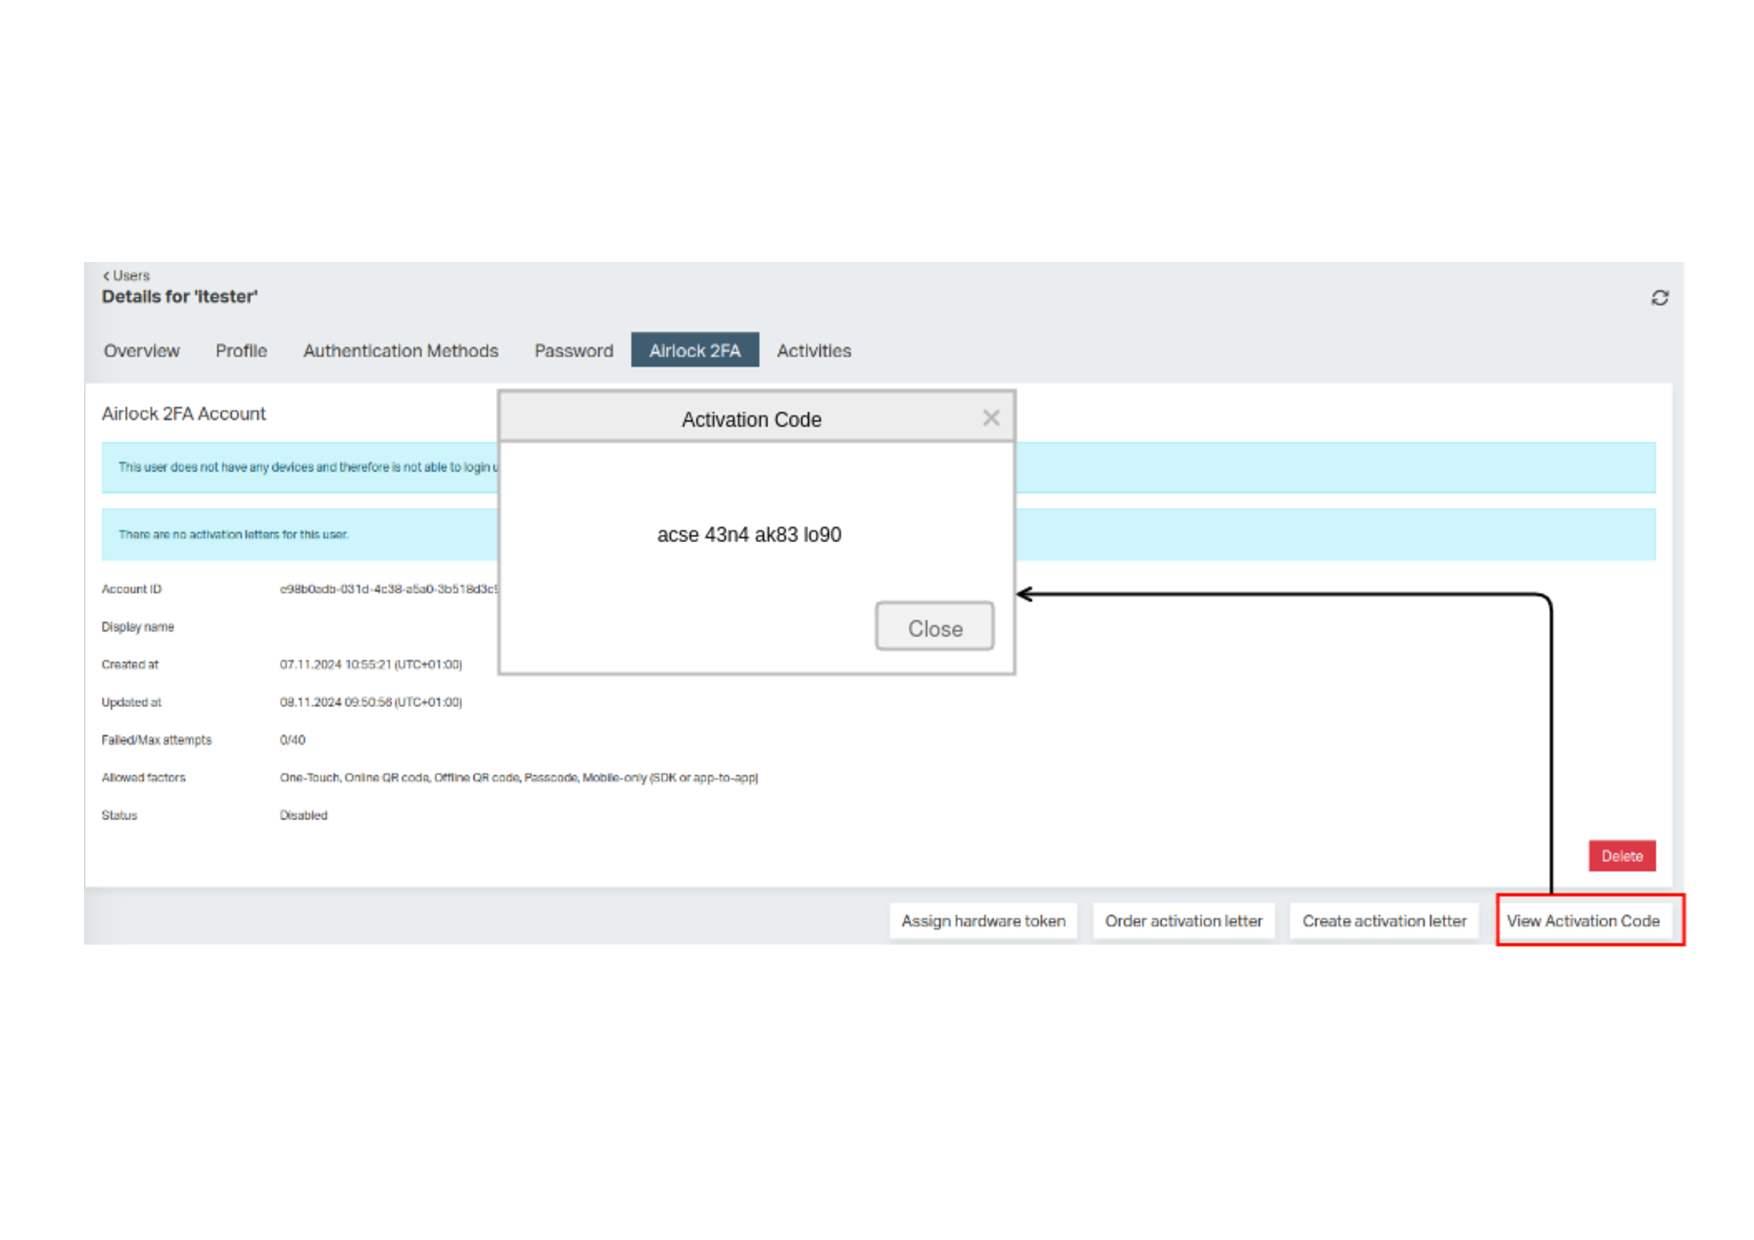
\includepdf[pages=-, angle=90]{ressourcen/Mockup1}
\end{landscape}
\noindent Es wird der Ansatz verfolgt, dass unten rechts ein weiterer Button hinzukommt. Dieser wird allerdings nur dann angezeigt, wenn der Admin auch die nötigen Rollen dazu hat und ein offener Aktivierungscode vorhanden ist(sprich nicht null zurück kommt). Wird der Button geklickt, soll sich ein Popup öffnen, in dem der 16-stellige Aktivierungscode angezeigt wird. Ev. könnte es auch eine Option sein, das Enrollmentdatum auch noch anzuzeigen, das könnte bei Fehlversuchen dem Admin eventuell hilfreich sein. Dies könnte dann in etwa so aussehen:
\begin{figure}[H]
	\begin{center}
		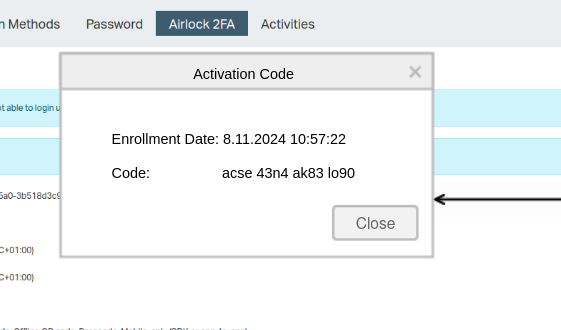
\includegraphics[width=0.8\textwidth]{ressourcen/popup}
		\caption[Popup mit Datum]{Popup Variante mit Datum}\label{fig:popupvariant}
	\end{center}
\end{figure}

\subsection{Lösungsvariante ohne Popup}
Anstelle eines Popups, welches durch einen Button ausgelöst wird, könnte man in der Accountübersicht auch folgendes einbauen:
\begin{figure}[H]
	\begin{center}
		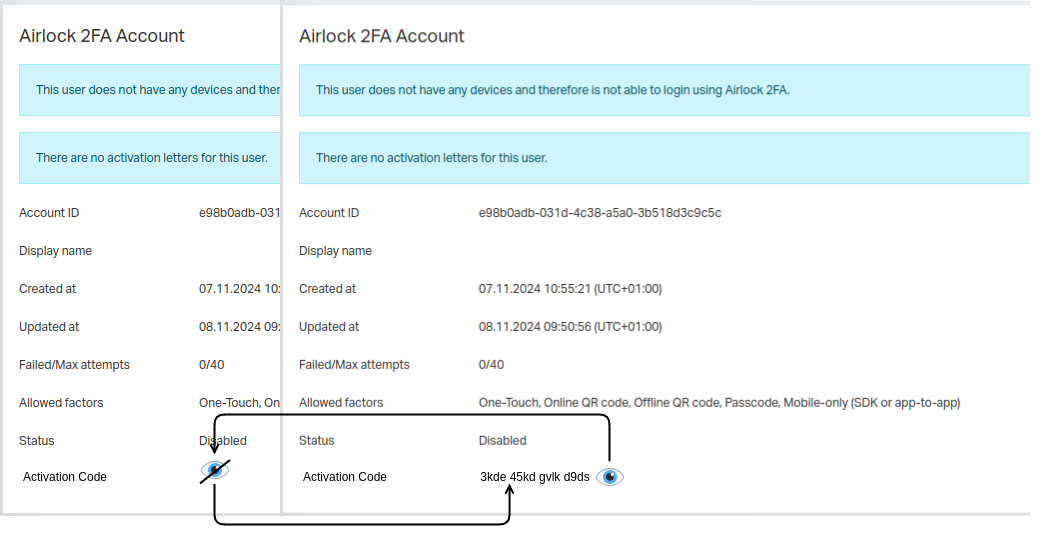
\includegraphics[width=1.0\textwidth]{ressourcen/variant_2_spa}
		\caption[Variante ohne Popup]{SPA Lösung ohne Popup}\label{fig:withoutpopup}
	\end{center}
\end{figure}
\noindent Analog zu einer Passwortanzeige könnte man es mit einem Auge darstellen. Wird auf das durchgestrichene Auge geklickt, wird der Code angezeigt. Klickt man nun auf das offene Auge, verschwindet der Aktivierungscode wieder.\newline
Diese neue Zeile wird nur dann angezeigt, wenn auch ein Aktivierungscode vorhanden ist und der Admin die erforderlichen Rechte hat.

\subsection{Rollenlogik}
Damit sichergestellt wird, dass der Button nur dann angezeigt wird, wenn der Benutzer dies möchte, kann ihm das Attribut \flqq hideOnAccessDenied\frqq{} gesetzt werden. Der Button braucht zudem ein sprechende ID. Diese ID wird dann im Access Controller im Backend, als Permissonkey verwendet.

\subsection{Wichtige Komponenten und Services}
\begin{itemize}
	\item airlock-2fa.component.html: In diesem File wird die Darstellung des UI definiert. Hier muss der neue Button hinzugefügt werden.
	\item airlock-2fa.service.ts: In diesem Service wird der Request an das IAM-Backend gemacht, um den Aktivierungscode zu bekommen. Anschliessend wird die Response geparsed und zurückgegeben.
	\item airlock-2fa.component.ts: In dieser Component, wird die Logik für den neuen Button implementiert. Konkret:
	\begin{itemize}
		\item Beim laden der Komponente wird via den obigen Service, der Aktivierungscode abgefragt.  
		\item Er darf nur angezeigt werden, falls auch ein Aktivierungscode vorhanden ist. Dies kann über die Response des Backends ermittelt werden, ist sie leer, existiert keine anstehende Aktivierung.
		\item Wird er angeklickt, öffnet sich ein Popup mit dem aktuellsten, offenen, 16-stelligen Aktivierungscode.
	\end{itemize}
	\item Zudem wird es ein neues Model für den Aktivierungscode geben müssen, falls das Datum auch angezeigt werden soll. Das sollte wie folgt aussehen:
		\begin{lstlisting}[language=TypeScript]
export interface Airlock2FAActivationCodeData {
		activationCodeShort: string;
		enrollmentDate: Date;
}
		\end{lstlisting}
\end{itemize}
\subsection{Translation Keys}
Um in der Adminapp die Sprachen Deutsch, Englisch und Französisch zu unterstützen wird i18n verwendet. Dafür wird für jeden String in der SPA ein Translation Key definiert. Hierfür gibt es 3 verschiedene JSON-Files; für jede Sprache eines. Das Value ist der übersetzte Text in die jeweilige Sprache. Je nach Sprache wird nun ein anderes JSON-File angezogen, dies führt dazu, dass immer die korrekte Übersetzung verwendet wird. In diesem Fall benötigt es mindestens folgende 3 Keys:
\begin{itemize}
	\item user.airlock-2fa.activation.view-activation-code.button: Text im Button
	\item user.airlock-2fa.activation.view-activation-code.popup.title: Titel des Popup's
	\item user.airlock-2fa.activation.view-activation-code.popup.text: Text im Popup
\end{itemize}

\section{Testkonzept} \label{sec:testkonzept}
Das neue Feature soll fehlerfrei und sowie in den Anforderungen definiert, funktionieren. Um dies Sicherzustellen wird folgend ein Testkonzept zusammen gestellt, nach welchem das Feature später getestet werden sollte.
Alle erwähnten Technologien sind in Kapitel \ref{sec:verwendete-tools} verlinkt.

\subsection{Benötigte Testmittel}
Unit-Tests und sämtliche Integration-Tests werden von der Entwicklungsumgebung Intellij ausgeführt. Da die Applikation lokal auch aus dem Intellij gestartet werden kann, werden auch die manuellen Tests mit der Hilfe von Intellij durchgeführt. Die Applikation läuft dann auf dem Port 8443. \newline
\\
Damit sichergegangen werden kann, dass nicht nur das neue Feature funktioniert, sondern alles darum herum auch noch, führt die Jenkinspipline bei jedem Push eines neuen Patchsets eine Auswahl an Tests aus.
\subsection{Wiremock} \label{subsec:wiremock}
In gewissen Unit- sowie allen Integration-Tests wird Wiremock verwendet um den Futurae Server zu simulieren. Wiremock stellt dabei einen Dummy-Server zurverfügung, das heisst alle Anfragen gehen an diesen Server und somit nicht über das Netzwerk. Dies verhindert Flaky Tests und bietet eine konstante und auf den Testcase angepasste API. Denn, dieser Server wird für jeden Test individuell konfiguriert.

\subsection{Unit-Tests}
Unit-Tests werden verwendet, um die Kernlogik in kleinen isolierten Einheiten zu testen. Hierfür werden komplexe Umsysteme und Klassen gemockt. Für die Klassen wird dies mit Mockito gemacht. Die Tests ansich werden mit JUnit5 implementiert. Konkret für diesen Auftrag müssen folgende Kernfunktionalitäten mit Unit-Tests abgedeckt werden:
\begin{itemize}
	\item Check, ob ein Admin die richtigen Rollen besitzt.
	\item Die neue Funktion im FuturaeAdminApiEnrollmentServiceImpl.java welche den neusten, offenen Aktivierungscode zurück gibt:
	\begin{itemize}
		\item Verhalten im Fehlerfall
		\item Verhalten im Erfolgsfall
		\item Verhalten im Erfolgsfall aber ohne ausstehender Aktivierung
	\end{itemize}
	\item Die neue Methode im Airlock2FAAdminService.java inkl. dem Logging.		
\end{itemize}

\subsection{REST-Integration-Tests}
Die REST-Integration-Tests werden auch mit hilfe von JUnit geschrieben. Anderst als bei den Unit-Tests wird hier nicht eine kleine Einheit getestet sondern der ganze Teil von der REST-Resource bis zur Datenbank.
Mit den Integration-Tests wird sicher gestellt, dass das ganze Feature im Backend richtig funktioniert. Für das sind folgende zwingende Fälle zu testen:

\begin{itemize}
	\item Es dürfen nur berechtigte Admins den Code erhalten, resp. Zugriff auf den neuen Endpunkt haben.
	\item Es muss eine 403 Response zurück kommen, wenn ein Admin nicht berechtigt ist.
	\item Falls kein offenes Enrollment existiert, der Admin aber berechtigt wäre, muss die Response leer sein.
\end{itemize}

\subsection{UI-Integration-Tests}
Zusätzlich zu den Rest-Integration-Tests werden auch UI-Integration-Tests erstellt. Diese Tests werden mit Selenium ausgeführt. Mit ihnen wird das UI / die SPA im Zusammenspiel mit dem IAM-Backend getestet.
Folgende fälle sind zu Testen:
\begin{itemize}
	\item Hat der Admin keine Berechtigung, darf der Button gar nicht erst angezeigt werden.
	\item Hat der Admin die Berechtigung, es gibt jedoch keinen Activation Code, darf der Button auch nicht angezeigt werden.
	\item Hat der Admin die Berechtigung und es ist ein Activation Code vorhanden, muss der Button angezeigt werden.
	\item Wird der Button geklickt muss ein Popup aufgehen, in welchem der Activation Code steht.
	\item Klickt man in diesem Popup auf <<Schliessen>>, sollte man wieder auf der Airlock 2FA Mangamentseite landen.
\end{itemize}
\newpage

\subsection{Manuelle Tests} \label{subsec:mtests}
Die Funktionalitäten werden durch die vielen automatisierten Tests schon ziemlich gut getestet. Allerdings ist es auch wichtig, das ganze manuell zu Testen. Der wichtigste Grund ist, dass der Futurae Server nicht mehr gemockt ist, sondern nun eine richtige Verbindung besteht. Damit es nicht zu unerwarteten Fehlern in Kombination mit Futurae kommt, sind diese Test sehr wichtig. Für die manuellen Tests sind folgende Testfälle definiert:

	\begin{longtable}{p{.25\textwidth}|p{.55\textwidth}}
	\hline
	\textbf{Testfall}    			& M1 \\
	\hline
	\textbf{Testumgebung}	& 
	\begin{itemize}
		\item IAM auf Localhost 
		\item Demokonfiguration ergänzt mit der Konfiguration des Futurae Service.
	\end{itemize}\\
	\hline
	\textbf{Beschreibung}   		& Der Admin hat die nötigen Rollen, damit er den Aktivierungscode ansehen kann und es gibt ein Enrollment welches offen ist. Der Admin klickt auf den Button, welcher ihm den Aktivierungscode anzeigen soll. \\
	\hline
	\textbf{Erwartetes Resultat}	& Es öffnet sich ein Popup (kein Browserpupop), mit dem Aktivierungscode und allenfalls dem Enrollmentdatum. \\
	\hline
	
\end{longtable} 
	\begin{longtable}{p{.25\textwidth}|p{.55\textwidth}}
	\hline
	\textbf{Testfall}    			& M2 \\
	\hline
	\textbf{Testumgebung}	& 
	\begin{itemize}
		\item IAM auf Localhost 
		\item Demokonfiguration ergänzt mit der Konfiguration des Futurae Service.
		\item Postman um Request ohne SPA abzusetzen
	\end{itemize}\\
	\hline
	\textbf{Beschreibung}   		& Der Admin hat die nötigen Rollen nicht, damit er den Aktivierungscode ansehen kann, es gibt aber ein Enrollment welches offen ist.\\
	\hline
	\textbf{Erwartetes Resultat}	& Der Button wird nicht angezeigt. Der Admin darf auch via einen alternativen REST-Client, wie z.B Postman, den Aktivierungscode nicht bekommen. \\
	\hline
	
\end{longtable} 
\newpage

\begin{longtable}{p{.25\textwidth}|p{.55\textwidth}}
\hline
\textbf{Testfall}    			& M3 \\
\hline
\textbf{Testumgebung}	& 
\begin{itemize}
	\item IAM auf Localhost 
	\item Demokonfiguration ergänzt mit der Konfiguration des Futurae Service.
\end{itemize}\\
\hline
\textbf{Beschreibung}   		& Der Admin hat die nötigen Rollen nicht, damit er den Aktivierungscode ansehen kann und es gibt kein Enrollment welches offen ist.\\
\hline
\textbf{Erwartetes Resultat}	& Der Button wird nicht angezeigt. \\
\hline

\end{longtable}  

\section{Qualitätssicherungskonzept}
Das Qualitätssicherungskonzept wird definiert, um eine möglichst hohe Qualität des Codes zu erhalten.
\newline
Die Qualität des Codes ist im IAM-Repository schon sehr gut erzwungen. Durch Architecture Layering Tests und Checkstyle sind IAM-Spezifische Vorgaben getestet, damit der Code einheitlich bleibt. Zusätzlich gibt es auch noch PMD und Spotbugs Checks. Die PMD Checks prüfen den Code auf unschönheiten, basierend auf IAM-spezifischen Regeln. Das selbe gilt für SpotBugs.
\newline
Durch all diese Tests wird die Qualität sehr gut sichergestellt. Bei jedem Push eines neuen Patchsets werden diese Checks, zusätzlich zu den normalen Tests, auch in der Jenkinspipeline ausgeführt.







